%%%%%%%%%%%%%%%%%%%%%%%%%%%%%%%%%%%%%%%%%%%%%%%
% BEGIN IMPULS
%%%%%%%%%%%%%%%%%%%%%%%%%%%%%%%%%%%%%%%%%%%%%%%
\chapter{Impuls}

In dit hoofdstuk wordt de wet van behoud van impuls uitgelegd en gaan we botsingen van objecten 
bestuderen. Zowel elastische als inelastische botsingen worden behandeld en de wet van behoud 
van energie blijkt ook hier een essentiele rol te spelen.

Stof uit Giancoli:
\begin{itemize}
\item Hoofdstuk 9.1-9.9
\end{itemize}

\section{Behoud van impuls} \label{sec:impuls}

We beschouwen in deze paragraaf nogmaals de $2^e$ en $3^e$ wet van Newton. Met
deze eenvoudige beschouwing komen we tot een van de belangrijkste behoudswetten 
in de natuur: het behoud van impuls. Samen met het behoud van energie zoals
we tegenkwamen in hoofdstuk~\ref{chap:energie} is dit een van de belangrijkste
wetten in de klassieke mechanica. Ook daarbuiten in de relativiteitstheorie en de 
quantummechanica zijn impuls en energie behouden grootheden: sterker nog, er zijn 
nog nooit natuurverschijnselen waargenomen waarbij deze behoudswetten worden
geschonden.

Laten we om te beginnen kijken naar een systeem van twee objecten waarop geen 
externe krachten worden uitgeoefend, terwijl de twee objecten wel een kracht op
elkaar kunnen uitoefenen. Nu weten we dankzij de $3^e$ wet van Newton dat:
\begin{equation}
\vec{F}_{A\rightarrow B}=-\vec{F}_{B\rightarrow A}
\end{equation}
De kracht die object $A$ op $B$ uitoefent is even groot als de kracht van $B$ op $A$, maar
tegengesteld van richting. Verder weten we dat een kracht resulteert in een verandering
van impuls. Dus:
\begin{eqnarray}
\frac{d\vec{p}_A}{dt} & = & -\frac{d\vec{p}_B}{dt}  \\
\frac{d}{dt}\left(\vec{p}_A+\vec{p}_B\right) & = & \vec{0} \\
&\Downarrow&\nonumber \\
\vec{p}_A+\vec{p}_B & =  & \vec{C}
\end{eqnarray}
Ofwel de totale impuls voor een 2-deeltjes systeem waarop geen externe krachten worden 
uitgeoefend is constant. Dit is een belangrijke observatie, waarvan in het begrijpen en 
doorrekenen van vele problemen gebruik kan worden gemaakt. Bovendien is het eenvoudig 
te bewijzen dat de wet van behoud van impuls geldt voor een willekeurig systeem van 
deeltjes, waarop geen netto externe kracht  werkt. Als we een systeem van $n$ objecten
bekijken kunnen we schrijven voor de totale impuls $\vec{P}$:
\begin{equation}\label{eq:ptot}
\vec{P} = \vec{p}_1 + \vec{p}_2 .... + \vec{p}_n = \sum_i^n\vec{p}_i
\end{equation}
En door te differentieren naar de tijd krijgen we:
\begin{equation}\label{eq:fsum}
\frac{d\vec{P}}{dt} = \sum_i^n\frac{d\vec{p}_i}{dt} = \sum_i^n \vec{F}_i
\end{equation}
waarbij $\vec{F}_i$ de netto kracht is op object $i$. Nu kunnen we een onderscheid 
maken tussen krachten die werken tussen twee van de objecten die we \emph{interne} krachten
noemen, en krachten die van buiten op ons systeem werken ofwel \emph{externe} krachten.
Nu gebruiken we wederom de $3^e$ wet van Newton: als er een object een interne kracht
ondervindt, is er een ander object in ons systeem dat een even grote kracht ondervindt
met tegengestelde richting. Netto dragen de interne krachten dus niet bij aan de
som in vgl.~\ref{eq:fsum}. We kunnen dus concluderen dat de impulsverandering
voor een systeem van objecten wordt gegeven door de som van externe krachten op dat systeem:
\begin{equation}\label{eq:atot}
\frac{d\vec{P}}{dt} = \sum \vec{F}_{ext}
\end{equation}
Als de som van externe krachten nul is, is de impuls van dat systeem dus constant. 
Merk trouwens wel op dat de externe krachten ook door 'iets' of 'iemand' moeten worden
uitgeoefend. Als die 'iets' of 'iemand' bij het systeem van objecten wordt meegenomen zal
de totale impuls van het totale systeem constant zijn.

\begin{center}
\line(1,0){250}
\end{center}
\begin{voorbeeld} \label{ex:bots1}
Een karretje met massa $m_A$ en snelheid $\vec{v}_A$ botst op een stilstaand karretje
met massa $m_B$. Na de botsing gaan de karretjes samen verder (mooi he). (i) Bereken de 
snelheid van de twee karretjes na de botsing (verwaarloos wrijving). (ii) Bereken de energie 
voor en na de botsing.

 \begin{figure}[htbp]
\begin{center}
  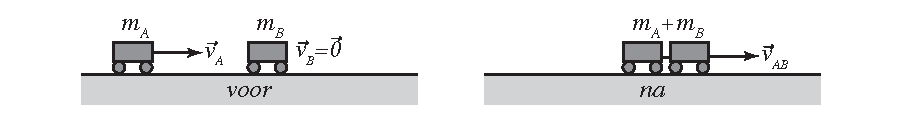
\epsfig{file=BotsVoorbeeld1.pdf, width=\textwidth}
\caption{{\it Twee botsende karretjes.}}
\label{fig:bots1}
\end{center}
\end{figure} 
{\bf Oplossing: }{\it (i) Er is geen netto externe kracht op onze twee karretjes, dus weten we dat de totale
impuls hetzelfde is voor en na de botsing. Laten we voor het gemak aannemen dat $\vec{v}_A$ langs
de $x$-as ligt. We hoeven dan slechts een 1-D vergelijking op te stellen voor impulsbehoud.
\begin{eqnarray}
\vec{P}_{voor} &= &\vec{P}_{na} \\ 
m_A \, |\vec{v}_A| & =& (m_A + m_B) \,|\vec{v}_{AB}|
\end{eqnarray}
Waaruit eenvoudig volgt dat:
\begin{equation}
|\vec{v}_{AB}| = |\vec{v}_A| \frac{m_A}{m_A+m_B}
\end{equation}
(ii) Laten we nou eens kijken naar de energie voor en na de botsing. Voor de botsing hebben
we alleen de kinetische energie van karretje $A$:
\begin{equation}
K_{voor} = \frac{1}{2}m_A\,|\vec{v}_A|^2
\end{equation}
En na de botsing:
\begin{eqnarray}
K_{na} & = & \frac{1}{2} (m_A+m_B) |\vec{v}_{AB}|^2 \\
& = & \frac{1}{2} \frac{m_A^2}{m_A+m_B} |\vec{v}_A|^2 \\
& < & K_{voor}
\end{eqnarray}
Het lijkt er op alsof energiebehoud is geschonden, omdat er na de botsing minder kinetische energie
is dan voor de botsing. Het is inderdaad zo dat er minder mechanische energie in het systeem zit. Een
deel van de energie is gedissipeerd (verbruikt) in het laten samengaan van de twee karretjes. Wat we
hier hebben gezien is een voorbeeld van een zogenaamde inelastiche botsing. In de volgende paragrafen
gaan we dieper in op de verschillende typen botsingen.
}
\end{voorbeeld}
\begin{center}
\line(1,0){250}
\end{center}

\section{Zwaartepunt systeem}

Het is instructief om op een meer formele manier aan te kijken tegen de discussie over impulsbehoud
uit de vorige paragraaf. Voor analyses van meer-deeltjes systemen wordt namelijk meestal expliciet een
onderscheid gemaakt tussen de beweging van het systeem als geheel en de beweging van de deeltjes
- of objecten - die het systeem zelf vormen. Daarvoor wordt gekeken naar de beweging van het zwaartepunt
van het systeem, en de beweging van de objecten ten opzichte van het zwaartepunt.

Het zwaartepunt of massa-middelpunt van een systeem van deeltjes wordt gegeven door:
\begin{equation}
\vec{r}_{CM} \equiv \frac{\sum_i m_i \vec{r}_i}{\sum_i m_i} = \frac{\sum_i m_i \vec{r}_i}{M}
\end{equation}
Hierin is $M$ de totale massa van het systeem van objecten. Het onderschrift $CM$ van $\vec{r}_{CM}$ komt
van het Engelse woord voor massa-middelpunt, 'center-of-mass'. Om te onderzoeken hoe nou 
het $CM$ beweegt kunnen we om te beginnen eens de snelheid van het  $CM$ uitrekenen, ofwel:
\begin{equation}
\vec{v}_{CM} \equiv \frac{d\vec{r}_{CM}}{dt} = \frac{1}{M}\,\sum_i m_i \frac{d\vec{r}_i}{dt} = \frac{1}{M}\,\sum_i \vec{p}_i 
\end{equation} 
De laatste som uit deze vergelijking bevat de totale impuls zoals we die hebben gedefinieerd
in vgl.~\ref{eq:ptot} en we hebben nu een eenvoudig verband tussen de zwaartepunt beweging en 
de totale impuls van een systeem. De totale massa van een systeem maal de snelheid van het
zwaartepunt is gelijk aan de totale impuls. We kunnen nu ook eens kijken hoe de impuls van een systeem
van deeltjes eruit ziet als je 'meereist' met het zwaartepunt. We kunnen de coordinaten van onze
objecten dan herdefinieren als:
\begin{equation}
\vec{r}_i\rightarrow\vec{r}_i^{'} = \vec{r}_i-\vec{r}_{CM}
\end{equation}
De impuls die een object heeft als je meereist met het zwaartepunt wordt dan gegeven
door (\emph{laat zien.}):
\begin{equation}
\vec{p}_i^{'} = \vec{p}_i - \frac{m_i}{M}\vec{P}
\end{equation}
Op het eerste geizcht lijkt deze uitdrukking niet echt ergens goed voor, maar we kunnen nu eens kijken
naar de som van impulsen in het zwaartepuntssysteem. Hiervoor geldt:
\begin{eqnarray}
\sum_i \vec{p}_i^{'} & = & \sum_i \left(\vec{p}_i - \frac{m_i}{M}\vec{P}\right) \\
& = & \vec{P} - \frac{M}{M}\vec{P} \\
& = & \vec{0}
\end{eqnarray}
Dus het totale impuls ten opzichte van het zwaartepunt is gelijk aan $\vec{0}$ en deze som verandert 
ook niet als functie van de tijd. Dit resultaat wordt vaak gebruikt voor analyse van bijvoorbeeld botsingen:
berekeningen worden in eerste instantie uitgevoerd in het $CM$ systeem. De snelheden van objecten 
kunnen vervolgens weer 'getransformeerd' worden naar het lab-systeem door daar eenvoudig de snelheid
van het zwaartepunt bij op te tellen.

We kunnen nu nog een stap verder gaan en eens kijken hoe de versnelling van het zwaartepunt
eruit ziet:
\begin{eqnarray}
\vec{a}_{CM} & \equiv & \frac{d^2\vec{r}_{CM}}{dt^2} \\
& = & \frac{1}{M}\frac{d\vec{P}}{dt} \\
& = & \frac{1}{M}\sum \vec{F}_{ext}
\end{eqnarray}
Ofwel de versnelling van het zwaartepunt van een systeem van deeltjes is gelijk aan de
som van externe krachten gedeeld door de totale massa van het systeem. Met andere woorden
de beweging van het zwaartepunt van een systeem wordt volkomen geregeerd door de externe
krachten die erop werken, ongeacht wat de objecten in het systeem onderling met elkaar 
uitspoken.

\begin{center}
\line(1,0){250}
\end{center}
\begin{voorbeeld} \label{ex:cm1}
Een granaat van massa $M$ wordt afgeschoten zoals getekend in Fig.~\ref{fig:cm1}: de 
snelheid op $t=0$ is $\vec{v}_0$ en de hoek van afvuren is $\theta_0$. Op het hoogste punt
valt de granaat uiteen in twee stukken: een van $3/4\,M$ en een van $1/4\,M$. Het stuk van
$3/4M$ komt neer op afstand $h_0$.  (i) Geef een uitdrukking voor de afstand $h_1$ die het andere 
stuk aflegt. (ii) Wat is de relatieve snelheid van de twee stukken op het moment van de explosie?

\begin{figure}[htbp]
\begin{center}
  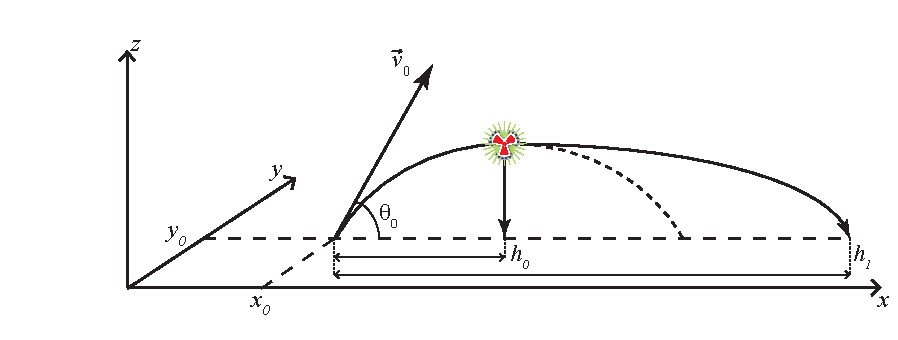
\epsfig{file=CMVoorbeeld1.pdf, width=\textwidth}
\caption{{\it Exploderende granaat.}}
\label{fig:cm1}
\end{center}
\end{figure} 
{\bf Oplossing: }{\it (i) De granaat ontploft op het hoogste punt van zijn baan, en de snelheid 
in de $z$-richting is op dat moment 0. We weten dat beide fragmenten van de granaat dus
gelijk de grond raken. Totdat de fragmenten de grond raken beschrijft het zwaartepunt van de
twee granaatscherven een paraboolbaan, omdat de enige externe kracht de zwaartekracht is.
Aangezien $h_0$ precies ligt op de helft van de afstand die het zwaartepunt aflegt, bevindt het
zwaartepunt zich op $x_{CM}=2\,h_0$ als beide fragmenten de grond raken. We hebben dus
de volgende vergelijking:
\begin{eqnarray}
x_{CM} &  =  & \frac{\sum_i m_i x_i}{\sum_i m_i} \\
& \Downarrow & \\
2\,h_0 & = & \frac{1}{M}\left(\frac{3}{4}M\,h_0 +\frac{1}{4}M\,h_1\right)
\end{eqnarray}
Hieruit kunnen we $h_1$ oplossen:
\begin{equation}
h_1 = 5\,h_0
\end{equation}
(ii) Op het tijdstip van exploderen heeft de granaat een snelheid:
\begin{equation}
\vec{v}(CM) = (|\vec{v}_0|\cos\theta,\,0,\,0)
\end{equation}
In het $CM$ systeem heeft het fragment met $m=3/4\,M$ op het moment van exploderen een 
snelheid van $\vec{v}(1)=-\vec{v}(CM)$, 
want in het niet bewegende referentie-frame staat het fragment immers stil. Nu kunnen we de snelheid
van het andere fragment in het $CM$ systeem oplossen omdat $\sum_i \vec{p}_i (CM) = \vec{0}$. Dus
voor de $x$-component van de impuls in het $CM$ systeem geldt:
\begin{eqnarray}
0 & = & -\frac{3}{4}\,M\,v(CM)_x+\frac{1}{4}\,M\,v(2)_x \\
&\Downarrow &\\
v(2)_x & = & 3\,v(CM)_x
\end{eqnarray}
Dus de relatieve snelheid van de twee fragmenten is:
\begin{equation}
\vec{v}(2) -\vec{v}(1) = (4|\vec{v}_0|\cos\theta_0,\,0,\,0)
\end{equation}
En het aardige is dat de relatieve snelheid in beide referentiesystemen hetzelfde is (\emph{laat zien}).
}
\end{voorbeeld}
\begin{center}
\line(1,0){250}
\end{center}

\section{Elastische botsingen}

We hebben aan het einde van paragraaf~\ref{sec:impuls}  een voorbeeld gezien
van een inelastische botsing, maar we gaan studie van botsingen beginnen met botsingen
waarvoor de kinetische energie voor en na de botsing hetzelfde is. Dus:
\begin{eqnarray}
\sum \vec{P}_{voor} & =  & \sum \vec{P}_{na} \\
\sum K_{voor} & = & \sum K_{na}
\end{eqnarray}
Zulke botsingen waarbij de kinetische energie naast impuls is behouden heten elastische
botsingen. Je moet je wel realiseren dat de kinetische energie niet gedurende het hele
botsingsproces is behouden. Denk bijvoorbeeld aan het frontaal botsen van twee perfecte gelijke 
stuiterballen: voor en na de botsing hebben de ballen evenveel kinetische energie, maar op het
moment van botsen komen beide ballen even tot stilstand en wordt de kinetische energie voor
een korte tijd 'opgeslagen' als potentiele energie (in dit geval een vorm van veerenergie). De 
totale impuls is gedurende de hele botsing uiteraard wel constant vanwege Newton's $3^e$~wet.
 
 \begin{figure}[htbp]
\begin{center}
  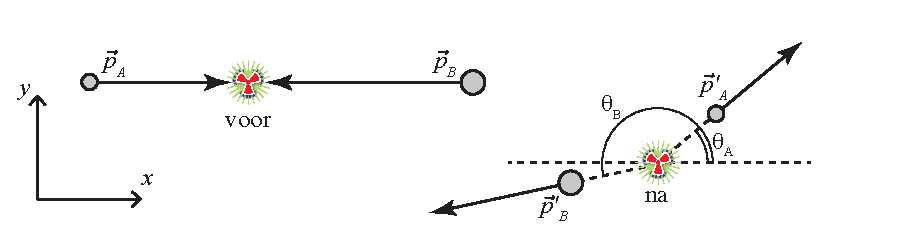
\epsfig{file=Botsing2D.pdf, width=\textwidth}
\caption{{\it Botsende objecten in 2-D.}}
\label{fig:bots2d}
\end{center}
\end{figure} 
In het geval van een twee deeltjes botsing gaan we nu de vergelijkingen voor impuls en energiebehoud
expliciet opschrijven. Laten we een deeltje $A$  botsen op een deeltje $B$ met initiele impulsen 
$\vec{p}_A$ en $\vec{p}_B$. De snelheden na de botsing worden gegeven door $\vec{p}_A^{\prime}$ en
$\vec{p}_B^{\prime}$ zoals aangegeven in Fig.~\ref{fig:bots2d}. Er geldt nu:
\begin{eqnarray}\label{eq:epbehoud}
\vec{p}_A +\vec{p}_B & = & \vec{p}_A^{\prime} + \vec{p}_B^{\prime} \\
\frac{|\vec{p}_A|^2}{2\,m_A}+\frac{|\vec{p}_B|^2}{2\,m_B} & = & \frac{|\vec{p}_A^{\prime}|^2}{2\,m_A}+\frac{|\vec{p}_B^{\prime}|^2}{2\,m_B}
\end{eqnarray}
Voor de laatste vergelijking is de kinetische energie herschreven als $\frac{1}{2}m|\vec{v}|^2 = \frac{|\vec{p}|^2}{2m}$. 
We kunnen impulsbehoud expliciet uitschrijven voor de $x$ component:
\begin{eqnarray}\label{eq:bots_px}
p_{Ax} + p_{Bx} & = & p_{Ax}^{\prime} + p_{Bx}^{\prime} \\
                             & = & |\vec{p}_A^{\prime}|\cos\theta_A + |\vec{p}_B^{\prime}|\cos\theta_B
\end{eqnarray}
Voor de $y$ component:
\begin{eqnarray}\label{eq:bots_py}
p_{Ay} + p_{By} & = & p_{Ay}^{\prime} + p_{By}^{\prime} \\
                          0 & = & |\vec{p}_A^{\prime}|\sin\theta_A + |\vec{p}_B^{\prime}|\sin\theta_B
\end{eqnarray}
Samen met de vergelijking voor behoud van energie heb je nu dus 3~vergelijkingen met
4~onbekenden: $|\vec{p}_A^{\prime}|$, $\vec{p}_B^{\prime}|$, $\theta_A$ en $\theta_B$. Er zit dus een 
bepaalde vrijheid in de verstrooing van twee objecten, maar op het moment dat bijvoorbeeld een van de twee 
hoeken wordt vastgelegd door bijvoorbeeld een meting, liggen de andere grootheden ook vast.

\begin{center}
\line(1,0){250}
\end{center}
\begin{voorbeeld} \label{ex:bots2}
Laten we nog eens kijken naar de botsing zoals weergegeven in Fig.~\ref{fig:bots2d}. Wat zijn
de impulsen $\vec{p}_A^{\prime}$ en $\vec{p}_B^{\prime}$ als $\theta_A=0$?

{\bf Oplossing: }{\it De $y$ component van de impulsen van beide objecten is eenvoudig te berekenen,
aangezien $\theta_A=0$. Door gebruik te maken van vgl.~\ref{eq:bots_py} zie je namelijk dat ook
$\theta_B=0$ of $\theta_B=\pi$ (twee oplossingen?), anders is impuls in de $y$ richting niet behouden. 
Verder weten we dat $|\vec{p}_{A,B}|=p_{Ax,Bx}$
omdat de impuls alleen een component in de $x$ richting heeft.  Vergelijkingen~\ref{eq:epbehoud} reduceren
dus tot:
\begin{eqnarray}
p_{Ax}+p_{Bx} & = & p_{Ax}^{\prime}+p_{Bx}^{\prime} \\
\frac{p_{Ax}^2}{m_A}+\frac{p_{Bx}^2}{m_B} & = & \frac{p_{Ax}^{\prime 2}}{m_A}+\frac{p_{Bx}^{\prime2}}{m_B}
\end{eqnarray}
Dit zijn twee vergelijkingen met twee onbekenden, $p_{Ax}^{\prime}$ en $p_{Bx}^{\prime}$, die we prima
kunnen oplossen. We kunnen bijvoorbeeld $p_{Ax}^{\prime} = p_{Ax}+p_{Bx}-p_{Bx}^{\prime}$ uit de impulsbehoud
vergelijking invullen in de vergelijking voor energiebehoud. We krijgen dan:
\begin{eqnarray}
\frac{p_{Ax}^2}{m_A}+\frac{p_{Bx}^2}{m_B} & = & \frac{\left(p_{Ax}+p_{Bx}-p_{Bx}^{\prime}\right)^2}{m_A}+\frac{p_{Bx}^{\prime2}}{m_B} \\
p_{Ax}^2+\frac{m_A}{m_B} p_{Bx}^2 & = &  p_{Ax}^2+p_{Bx}^2+2p_{Ax} p_{Bx}-2p_{Bx}^{\prime}(p_{Ax}+p_{Bx})+p_{Bx}^{\prime2} +\frac{m_A}{m_B}p_{Bx}^{\prime2}\\
0 & = & p_{Bx}^{\prime2}\left(1+\frac{m_A}{m_B}\right)-2\,p_{Bx}^{\prime}(p_{Ax}+p_{Bx})+p_{Bx}^2(1-\frac{m_A}{m_B})+2\,p_A\,p_B
\end{eqnarray}
Deze algebra is natuurlijk geen pretje, maar we kunnen het uiteraard wel oplossen. We hebben namelijk te
maken met een kwadratische vergelijking in $p_{Bx}^{\prime}$ en die kunnen we kraken met behulp van de
abc-formule. Voor $p_{Bx}^{\prime}$ vinden we (\emph{probeer, probeer, probeer}):
\begin{eqnarray}
p_{Bx}^{\prime} & = & \frac{(p_{Ax}+p_{Bx})\pm(p_{Ax}-\frac{m_A}{m_B} p_{Bx})}{1+\frac{m_A}{m_B}}\\
&\Downarrow &\\
p_{Bx}^{\prime} = p_{Bx} & \vee & p_{Bx}^{\prime} = \frac{2\,p_{Ax}+p_{Bx}(1-\frac{m_A}{m_B})}{1+\frac{m_A}{m_B}}
\end{eqnarray}
Wonderlijk dat er twee oplossingen zijn, net als voor $\theta_B$, maar bij nader inzien toch niet zo heel erg vreemd.
De eerste oplossing waarbij $p_{Bx}$ niet verandert correspondeert namelijk met een situatie waarin de
twee objecten elkaar niet raken. Nogmaals: deze rekenpartij was geen pretje en op deze manier ook geen onderdeel van
een tentamen.
}
\end{voorbeeld}
\begin{center}
\line(1,0){250}
\end{center}

Een alternatief op het stug doorrekenen van botsingen zoals in voorbeeld~\ref{ex:bots2} is de botsing te bekijken in 
het $CM$ systeem: je gaat dan als het ware 'meelopen' met het systeem van deeltjes zodanig dat de totale impuls
nul wordt. De eerste stap is dan het  berekenen van de snelheid van het $CM$ systeem:
\begin{equation}
\vec{v}_{CM} = \frac{1}{M}(\vec{p}_A + \vec{p}_B)
\end{equation}
Vervolgens kan je kijken hoe de impulsen van de objecten $A$ en $B$ eruit zien in het $CM$ systeem. Als we de
impulsen in het $CM$ systeem $\vec{k}_A$ en $\vec{k}_B$ noemen dan geldt:
\begin{eqnarray}
\vec{k}_{A,B} & = & m_{A,B}\,(\vec{v}_{A,B}-\vec{v}_{CM}) \\
                        & = & \mu (\vec{v}_{A,B} - \vec{v}_{B,A}) 
\end{eqnarray}
Waarbij we een nieuwe grootheid $\mu$ hebben geintroduceerd die bekend staat als 'gereduceerde massa'. Deze
is dus gedefinieerd als:
\begin{equation}
\mu \equiv \frac{m_A m_B}{m_A + m_B}
\end{equation}
De gereduceerde massa wordt vaak gebruikt in het beschrijven van botsingsprocessen. Het aardige van het
uitdrukken van de impulsen in termen van $\mu$ is dat je expliciet kan zien dat de som van impulsen in het
$CM$ systeem gelijk is aan nul omdat $\vec{k}_A=-\vec{k}_B$. Aangezien de som van de impulsen voor en na
de botsingen hetzelfde moet zijn, vanwege de wet van behoud van impuls, geldt na de botsing 
$\vec{k}_A^{\prime}=-\vec{k}_B^{\prime}$. Tenslotte weten we dat $|\vec{k}_A|=|\vec{k}_B|=|\vec{k}_A^{\prime}|=|\vec{k}_B^{\prime}|$
omdat we hier te maken hebben met een elastische botsing. 

Nu moeten we een keuze maken voor de hoek van verstrooing $\theta_{CM}$ in het $CM$ systeem, waarna
de momenta $\vec{k}_{A,B}^{\prime}$ vastgelegd zijn in het $CM$ systeem. De vrijheid van het kiezen van de verstrooingshoek
hebben we nog steeds, net als in het oorspronkelijke geval. Het enige wat ons nog rest is om de impulsen terug te 
transformeren naar het oorspronkelijk systeem - ook wel lab systeem genoemd. Dus:
\begin{equation}\label{eq:naarlab}
\vec{p}_{A,B}^{\prime} = \vec{k}_{A,B}^{\prime} + m_{A,B} \vec{v}_{CM}
\end{equation}
Wat we hebben gedaan is dus eerste de $CM$ snelheid van alle snelheden afhalen, vervolgens hebben we 
de botsing doorgerekend, en tenslotte zijn we naar het lab-systeem teruggekeerd. Procedureel lijkt deze methode 
lastig, maar het rekenwerk voor moeilijke problemen reduceert vaak aanzienlijk, zoals we zien in het volgende 
voorbeeld.

\begin{center}
\line(1,0){250}
\end{center}
\begin{voorbeeld} \label{ex:bots3}
Laten we nog eens kijken naar de botsing zoals weergegeven in Fig.~\ref{fig:bots2d}. Wat zijn
de impulsen $\vec{p}_A^{\prime}$ en $\vec{p}_B^{\prime}$ als $\theta_A=0$? Gebruik nu
de methode waarbij je eerst de botsing bekijkt in het $CM$ systeem.

{\bf Oplossing: }{\it Net als in voorbeeld~\ref{ex:bots2} kunnen we weer de $y$ component negeren. Voor
de botsing is er geen netto impuls in de $y$ richting, dus na de botsing ook niet. We hoeven dus weer alleen
te kijken naar de $x$ componenten van de impulsen en snelheden.

Voor de $CM$ snelheid geldt:
\begin{eqnarray}
v_{CM} & = & \frac{1}{M}(m_A v_{Ax} + m_B v_{Bx}) \\
& = & \frac{p_{Ax} + p_{Bx}}{M}
\end{eqnarray}
Voor de impulsen van $A$ en $B$ in het $CM$ systeem voor de botsing geldt:
\begin{eqnarray}
k_{Ax} & = & \mu (v_{Ax} - v_{Bx}) \\
k_{Bx} & = & \mu (v_{Bx} - v_{Ax}) 
\end{eqnarray}
Na de botsing geldt:
\begin{eqnarray}
k_{Ax}^{\prime} & = & \pm k_{Ax} \\
k_{Bx}^{\prime} & = & \pm k_{Bx} 
\end{eqnarray}
De oplossing met het $+$ teken corresponderen met een situatie waarin er geen botsing plaatsvindt. De
objecten $A$ en $B$ hebben elkaar gemist. De oplossingen met het $-$ teken horen bij botsende objecten.
We moeten nu weer terug naar het lab systeem. Met behulp van vgl.~\ref{eq:naarlab} krijgen we:
\begin{eqnarray}
p_{Bx}^{\prime} & = & -k_{Bx} + m_B v_{CM} \\
                             & = & -\frac{m_A m_B}{m_A+m_B} (v_{Bx} - v_{Ax}) + \frac{m_B}{m_A+m_B}(m_A v_{Ax} + m_B v_{Bx}) \\
                             & = & \frac{2p_{Ax} + p_{Bx}(1-\frac{m_A}{m_B})}{1+\frac{m_A}{m_B}}
\end{eqnarray}
Hetzelfde antwoord als in voorbeeld~\ref{ex:bots2}, maar wel met minder algebra gekregen. Probeer zelf een uitdrukking
te vinden voor $p_{Ax}^{\prime}$. De kans op fouten is op deze manier veel kleiner dan met de originele methode. 
Berekeningen van botsingsprocessen zijn bijna altijd het eenvoudigst in het $CM$ systeem.
}
\end{voorbeeld}
\begin{center}
\line(1,0){250}
\end{center}
\begin{voorbeeld} \label{ex:bots4}
Een object met massa $m$ botsts met impuls $\vec{p}_A$ op een stilstaand object $B$ met dezelfde massa. Na
de botsing is de observatie dat $\theta_A=-\theta_B=\pi/4$. (i) Bereken $\vec{p}_A^{\prime}$ (Hint: je hebt hiervoor alleen
impulsbehoud nodig). (ii) Is de botsing elastisch?

 \begin{figure}[htbp]
\begin{center}
  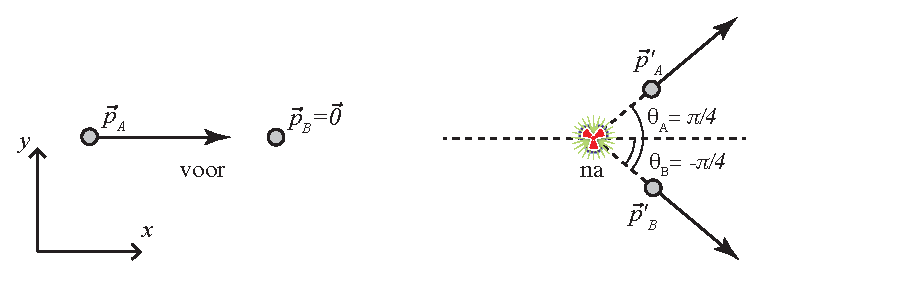
\epsfig{file=BotsVoorbeeld2.pdf, width=\textwidth}
\caption{{\it Botsing in 2-D: een object in rust ontmoet een even zwaar beest  dat niet in rust is.}}
\label{fig:BotsVoorbeeld2}
\end{center}
\end{figure} 

{\bf Oplossing: }{\it (i) Voor het oplossen van dit probleem is het niet nodig om eerst naar het $CM$ systeem
te gaan (maar het mag natuurlijk wel als je dat graag wil). Aangezien zowel hoek $\theta_A$ en $\theta_B$ vastliggen
hoef je alleen impulsbehoud te gebruiken om het probleem op te lossen: er zijn nog twee onbekenden, $|\vec{p}_A|$ en
$\vec{p}_B|$ en impulsbehoud geeft je twee vergelijkingen. Als niet alle vergelijkingen nodig zijn voor een 
oplossing dan is het systeem 'overbepaald': het kan dus gebeuren dat je niet aan alle vergelijkingen tegelijk kan 
voldoen. Impulsbehoud geeft je voor de $x$ component van de impuls:
\begin{eqnarray}
p_{Ax} & = & p_{Ax}^{\prime} + p_{Bx}^{\prime} \\
|\vec{p}_A| & = & |\vec{p}_A^{\prime}|\cos\theta_A +  |\vec{p}_B^{\prime}|\cos\theta_B \\
 & = & \frac{1}{\sqrt{2}}\left( |\vec{p}_A^{\prime}|+|\vec{p}_B^{\prime}|\right)\label{eq:bots4_1}
\end{eqnarray}
en voor de $y$ component:
\begin{eqnarray}
0 & = &  |\vec{p}_A^{\prime}|\sin\theta_A +  |\vec{p}_B^{\prime}|\sin\theta_B \\
   & = & |\vec{p}_A^{\prime}| -  |\vec{p}_B^{\prime}| \\
   & \Downarrow & \\
  |\vec{p}_A^{\prime}| & = & |\vec{p}_B^{\prime}|
\end{eqnarray}
Het laatste resultaat kunnen we invullen in vgl.~\ref{eq:bots4_1} waardoor we krijgen:
\begin{eqnarray}
|\vec{p}_A| & = & \frac{2 |\vec{p}_A^{\prime}|}{\sqrt{2}}\\
& \Downarrow & \\
|\vec{p}_A^{\prime}| & =  & \frac{|\vec{p}_A|}{\sqrt{2}}
\end{eqnarray}
(ii) Nu kunnen we kijken of ook de kinetische energie voor en na de botsing hetzelfde is gebleven.
Na de botsing is de kinetische energie gelijk aan:
\begin{eqnarray}
K_{na} & = &  \frac{|\vec{p}_A^{\prime}|^2}{2m} + \frac{|\vec{p}_B^{\prime}|^2}{2m} \\
& = & \frac{|\vec{p}_A|^2}{2m} \\
& = & K_{voor}
\end{eqnarray}
De kinetische energie is hetzelfde gebleven en de botsing is dus elastisch. Dit is toeval, want als
we de hoeken $\theta_{A,B}$ anders hadden gekozen was dit niet zonder meer het geval geweest.
}
\end{voorbeeld}

\section{Inelastische botsingen}

Het zal na de voorgaande discussie over elastische botsingen vast niet verbazen dat er ook
een klasse van botsingen bestaat waarbij de kinetische energie niet hetzelfde is voor en na 
de botsing. We hebben zelfs al zo'n  botsing gezien in voorbeeld~\ref{ex:bots1}. 
Voor een dergelijke botsing geldt dus voor de kinetische energie:
\begin{equation}
K_{na} - K_{voor} \neq 0
\end{equation}
Dit type botsing heet een inelastiche botsing. Het verschil in kinetische energie wordt ook
wel de $Q$ -waarde van het proces genoemd. Vaak verdwijnt er kinetische energie in een
in-elastische botsing en is $Q<0$, maar er zijn ook processen waarbij $Q>0$. Denk hierbij met name
aan het radioactieve verval van atoomkernen. Als je een kern in rust laat vervallen heb je
voor de 'botsing' geen kinetische energie, terwijl na de botsing de fragmenten van een kern dat wel
hebben.

Uiteraard is bij een in-elastische botsing de totale impuls voor en na de botsing wel hetzelfde.

\begin{center}
\line(1,0){250}
\end{center}
\begin{voorbeeld} \label{ex:bots5}
Bereken de $Q$-waarde van de botsende karretjes uit voorbeeld~\ref{ex:bots1}.

{\bf Oplossing: }{\it We hebben de kinetische energie voor de botsing:
\begin{equation}
K_{voor} = \frac{1}{2}m_A|\vec{v}_A|^2
\end{equation}
En na de botsing is de kinetische energie:
\begin{equation}
K_{na} = \frac{1}{2}\frac{m_A^2}{m_A+m_B}|\vec{v}_A|^2
\end{equation}
Voor de $Q$ waarde kunnen we dus schrijven:
\begin{eqnarray}
Q & = & K_{na}-K_{voor} \\
& = & \frac{1}{2}\left(\frac{m_A^2}{m_A+m_B} - m_A\right)|\vec{v}_A|^2\\
& = & -\frac{1}{2}\mu|\vec{v}_A|^2
\end{eqnarray}
Met $\mu$ de gereduceerde massa.
}
\end{voorbeeld}

\begin{center}
\line(1,0){250}
\end{center}

\begin{voorbeeld} \label{ex:bots6}
Een kogel met massa $m$ schiet in een blok hout met massa $M$ zoals getekend in Fig.~\ref{fig:BotsVoorbeeld3}. 
De maximale hoogte die het blok hout (plus de kogel) bereikt, is $h$. Wat was de snelheid van de kogel? 

\begin{figure}[htbp]
\begin{center}
  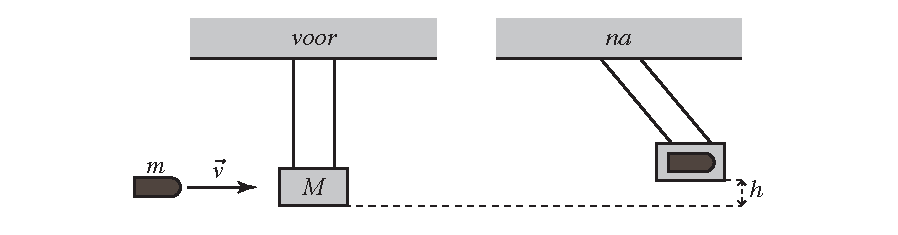
\epsfig{file=BotsVoorbeeld3.pdf, width=\textwidth}
\caption{{\it Ballistische slinger.}}
\label{fig:BotsVoorbeeld3}
\end{center}
\end{figure} 

{\bf Oplossing: }{\it Uit behoud van impuls weten we dat vlak na de inslag van de kogel in het blok hout
moet gelden:
\begin{eqnarray}
m|\vec{v} & = &(m+M) |\vec{v}^{\prime}| \\
& \Downarrow & \\
|\vec{v}^{\prime}| & = & \frac{m}{m+M}|\vec{v}| \label{eq:bots6_1}
\end{eqnarray}
Met $\vec{v}^{\prime}$ de snelheid van het blok plus de kogel.

Verder weten we dat de kinetische energie van het systeem wordt omgezet in
potentiele energie. Als het blok zijn maximale hoogte heeft bereikt is de $K$ gelijk nul. Dus:
\begin{eqnarray}
\frac{1}{2}(M+m)|\vec{v}^{\prime}|^2 & = & (M+m),g\,h \\
& \Downarrow & \\
|\vec{v}^{\prime}| & = & \sqrt{2\,g\,h}
\end{eqnarray}
Invullen van vgl.~\ref{eq:bots6_1} geeft:
\begin{equation}
|\vec{v}| = \frac{M+m}{m}\sqrt{2\,g\,h}
\end{equation}
}
\end{voorbeeld}

\begin{center}
\line(1,0){250}
\end{center}

%\section{Raketmakers formule}

\section{Wat moet ik weten en kunnen?}

Na dit hoofdstuk moet je weten:
\begin{itemize}
\item Waarom en onder wat voor omstandigheden impuls een behouden grootheid is.
\item Wat het zwaartepunt-systeem ($CM$) is.
\item Wat een elastische en in-elastische botsing is.
\end{itemize}
En je moet kunnen:
\begin{itemize}
\item Uitrekenen hoe het zwaartepunt van een systeem beweegt.
\item Berekenen wat de impulsen zijn na elastische en in-elastische 
botsingen van objecten.
\end{itemize}

\section{Opgaven}

\begin{enumerate}
\item Giancoli hoofdstuk~9. {\bf Problems}: 4, 15, 17, 18, 19, 36, 40, 41, 43, 49, 50, 56, 57, 58, 60, 
64, 66, 69, 72,  76, 79, 88, 90, 94, 100, 101, 102, 105, 112.
\item Je laat een object vallen. Het object gaat sneller bewegen dankzij de zwaartekracht. Is impuls
behouden, of niet? Leg uit.
\end{enumerate}
%%%%%%%%%%%%%%%%%%%%%%%%%%%%%%%%%%%%%%%%%%%%%%%
% EINDE IMPULS
%%%%%%%%%%%%%%%%%%%%%%%%%%%%%%%%%%%%%%%%%%%%%%%

